\documentclass[master=cws,masteroption=vs]{kulemt}
\setup{% Remove the "%" on the next line when using UTF-8 character encoding
  %inputenc=utf8,
  title={User attestation for the PinePhone},
  %Securing the PinePhone using ARM TrustZone while preserving the openness of the platform},
  author={Oberon Swings},
  promotor={Prof.\,dr.\,ir.\ F. Piessens},
  assessor={Prof.\,dr.\ D. Hughes \and Ir.\ P. Totis},
  assistant={Dr.\ J. M\"uhlberg \and Ir. F. Alder \and Ir. S. Pouyanrad}}
% Remove the "%" on the next line for generating the cover page
%\setup{coverpageonly}
% Remove the "%" before the next "\setup" to generate only the first pages
% (e.g., if you are a Word user).
%\setup{frontpagesonly}

% Choose the main text font (e.g., Latin Modern)
\setup{font=lm}

% If you want to include other LaTeX packages, do it here. 
\usepackage{csquotes}
\usepackage{pgfplots}
\pgfplotsset{width=10cm,compat=1.9}
\usepgfplotslibrary{external}
\tikzexternalize[mode=graphics if exists, figure list=true, prefix=TikzFigures/]
\graphicspath{{Figures/}}
% Finally the hyperref package is used for pdf files.
% This can be commented out for printed versions.
\usepackage[pdfusetitle,colorlinks,plainpages=false]{hyperref}

%\includeonly{chap-n}
\begin{document}

\begin{preface}
  TODO
\end{preface}

\tableofcontents*

\chapter*{Abstract}
TODO

\begin{abstract}
  TODO

\end{abstract}

% A list of figures and tables is optional
\listoffigures
%\listoftables
% If you only have a few figures and tables you can use the following instead
%\listoffiguresandtables
% The list of symbols is also optional.
% This list must be created manually, e.g., as follows:
\chapter{List of Abbreviations}
\section*{Abbreviations}
\begin{flushleft}
  \renewcommand{\arraystretch}{1.1}
  \begin{tabularx}{\textwidth}{@{}p{12mm}X@{}}
    IoT   	& Internet of Things \\
    TEE   	& Trusted Execution Environment \\
    I/O   	& Input and Output \\
    	OS		& Operating System
    	
  \end{tabularx}
\end{flushleft}
%\section*{Symbols}
%\begin{flushleft}
%  \renewcommand{\arraystretch}{1.1}
%  \begin{tabularx}{\textwidth}{@{}p{12mm}X@{}}
%    $c$   & Speed of light \\
%    $E$   & Energy \\
%    $m$   & Mass \\
%    $\pi$ & The number pi \\
%  \end{tabularx}
%\end{flushleft}

% Now comes the main text
\mainmatter

\documentclass{report}

\raggedright

\begin{document}

\chapter{Introduction}

\subsection*{Smartphones}

\paragraph*{Everyone} 
is assumed to have a smartphone of their own because it has become an essential gadget for our day to day lives.

\paragraph*{Everywhere}
these smartphones can be spotted, people use them at home, on the bus or even at work.

\paragraph*{Personal Computers}
seem less and less important to some people because all their needs can be fullfilled with a smartphone. 

\subsection*{Sensitive data}

\paragraph*{Making connections}
that is what these smartphone devices are good at but it is important to keep in mind that there are certain security implications with every connection that is made.

\paragraph*{Personal data}
is what drives the interactions with the smartphone. People use them to do online banking, send mails or even consult health related reports.

\subsection*{Related to IoT}

\paragraph*{Hardware similarities}
between smartphones and IoT devices are more prominent than one might expect. This is due to the fact that smartphones actually stem from IoT devices and not from personal computers.

\paragraph*{Security features}
for IoT devices is a hot research topic, this is because not many solutions or standards that are present today are found to be adequate in terms of protection against the existing threats.

\section{Problem statement}

\subsection*{IoT security}

\paragraph*{Performance}
is the main focus when IoT devices are designed, they only have a small number of tasks but these need to be executed as fast or as energy efficient as possible.

\paragraph*{Dynamic and distributed} 
groups of devices form an IoT network, this implies that the security of this network is as strong as the weakest link in the chain (which can be very weak in the IoT environment).

\subsection*{Progressive functionality}

\paragraph*{Banking, e-Health and mails}
are applications most people trust their smartphone with, even though personal computers weren't even trusted with these kinds of functionality a few decades ago.

\subsection*{Missmatch}

\paragraph*{Progressive functionality}
is what smartphones have been bringing for their users and is what makes that the industry keeps growing every year.

\paragraph*{Lagging or lacking security}
is the downside of this push for better functionality because it is very hard to make certain functionality secure but companies want to be the first to bring their products to the market.

\section{Contributions}

\paragraph*{Reproduction of existing work}
is the first goal of this thesis, the solution of the paper is replicated as closely as possible (no source code available). The experiments in the paper are redone to be able to make a comparison between the original and the implementation discussed here.

\paragraph*{Open source code}
is very important in the field of computer science because it allows other researchers to reproduce the experiments and review the work that has been done in a detailed manner.

\paragraph*{Extra experiment measurements}
are executed to expand on their work and give a more complete picture of the solution.

\paragraph*{Comparison with similar solutions}
is of course also important to evaluate whether this way of trying to solve the problem is in the right direction or whether different solutions have achieved more promising results.

\section{Outline}

In the next chapter more background information about among other things Remote Attestation and ARM TrustZone will be given. In the third chapter the methods to solve the problem will be explained. In chapter four the implementation of the attestation program are elaborated upon. In the fifth chapter the goal and outcome of the experiments will be made clear. The sixth chapter will conclude this thesis informing the reader about related work and future improvements. The final chapter will discuss the completed work.

\end{document}
\documentclass{report}

\raggedright

\begin{document}

\chapter{Background}

The smartphone that will be used is a PinePhone which is equiped with ARM TrustZone, it also comes with a component which can be used as Root of Trust to make secure boot possible. 

\section{Remote Attestation}

\begin{itemize}
\item Goal \begin{itemize}
\item Verify integrity
\end{itemize}
\item How it works \begin{itemize}
\item Verifier
\item Prover
\item Proof
\end{itemize}
\item Assumptions \begin{itemize}
\item Trusted third party
\item Secure keys
\end{itemize}
\end{itemize}

Remote attestation allows a device to prove to an external verifier that the software running on it is not tampered with. This attestation can go a lot further than this by for instance also checking the data structures on the device to make sure these are logical.

\section{Trusted Execution Environment}

\begin{itemize}
\item Execution \begin{itemize}
\item Isolation
\item Authentic code
\item Runtime integrity
\item Strict interfaces
\end{itemize} 
\item Trust \begin{itemize}
\item Static
\item Dynamic
\end{itemize}
\item Security \begin{itemize}
\item Data separation
\item Sanitization
\item Control of information flow
\item Fault isolation
\end{itemize}
\end{itemize}

A Trusted Execution Environment is a secure, integrity-protected processing environment, consisting of memory and storage capabilities.

\section{ARM TrustZone}

\begin{itemize}
\item Normal World \begin{itemize}
\item Rich OS
\end{itemize}
\item Secure World \begin{itemize}
\item Trusted Kernel
\item NS-bit
\item Secure Configuration Register
\end{itemize}
\item Peripherals \begin{itemize}
\item TZ Address Space Controller
\item TZ Protection Controller (interrupts)
\end{itemize}
\end{itemize}

ARM TrustZone is ARM's implementation of a TEE. This is achieved by having a secure and normal world in the System on Chip.

\section{PinePhone}

\begin{itemize}
\item Open source \begin{itemize}
\item
\end{itemize}
\item Linux \begin{itemize}
\item
\end{itemize}
\item ARM TrustZone \begin{itemize}
\item
\end{itemize}
\end{itemize}

The PinePhone is an open source smartphone which supports Linux as operating system which adds to it's openness.

\section{Secure boot, trusted boot and remote attestation for ARM TrustZone-based IoT Nodes}

\begin{itemize}
\item Solution \begin{itemize}
\item Overview
\end{itemize}
\item Trusted Boot \begin{itemize}
\item Trusted load phase
\item Attestation during boot
\end{itemize}
\item Remote attestation \begin{itemize}
\item Trusted execution time
\item Pagebased approach
\end{itemize}
\end{itemize}

\end{document}
\documentclass{report}

\raggedright

\begin{document}

\chapter{Method}

The main goal of this work is to achieve a secure open platform on the hardware.

\section{Detailed Problem}

\begin{itemize}
\item Lots of functionality \begin{itemize}
\item Sensitive data
\item Mobile computing
\end{itemize}
\item Performance driven \begin{itemize}
\item All resources to functionality
\item Little room for security
\item Extensive security measures needed
\end{itemize}
\item Hardware security solution \begin{itemize}
\item Security embedded in hardware
\item Better for performance
\item Correct implementation required
\end{itemize}
\end{itemize}

\section{System Model}

\begin{itemize}
\item Open platform \begin{itemize}
\item Multiple software providers
\item Platform owned by user
\end{itemize}
\item Secure software execution \begin{itemize}
\item Software isolation
\item Secure data storage
\end{itemize}
\end{itemize}

The system model describes an open platform with no or minimal trust among stakeholders.

\section{Attacker Model}

\begin{itemize}
\item Physical access \begin{itemize}
\item Threats
\item Vulnerabilities
\end{itemize}
\item OS/Firmware attacks \begin{itemize}
\item Threats
\item Vulnerabilities
\end{itemize}
\item Software attacks \begin{itemize}
\item Threats
\item Vulnerabilities
\end{itemize}
\end{itemize}

The attacker has physical access, can launch OS/firmware and software attacks. The Trusted Platform Module is assumed to be tamper resistent.

\section{Solution}

\begin{itemize}
\item Secure boot \begin{itemize}
\item Root of Trust
\item Chain of Trust
\item Secure starting point
\end{itemize}
\item User attestation \begin{itemize}
\item Integrity (control flow, data structures, ...)
\item Authenticity (code, ...)
\end{itemize}
\item Trust \begin{itemize}
\item Execution
\item Data protection
\end{itemize}
\end{itemize}

Ideally the device is started with secure boot, this makes sure the SW is started from a known secure state. 
\medskip

During operation the user should be able to attest whether their device is still in a secure state.
\medskip

This can be done using a TA that makes measurements on their device and reports back to them.
\medskip

These measurements are checking the integrity of the code section of the running applications and OS.

\end{document}
\chapter{Implementation}

\paragraph*{}
The goal of the implementation is to guarantee that the executable memory pages that are loaded into the memory are not tampered with. In general, this is achieved through RA where the device proves its trustworthiness to a remote verifier, in this case, it is the trusted base of the device itself that checks the integrity of the REE. This integrity check is achieved by measuring the code pages of the processes in advance, for instance, during the installation of the particular code. This measurement can be done in a variety of ways. In this thesis, hashing was chosen because of its common use and it being well understood by the community. After these initial measurements have been taken, they need to be stored in a secure place. The secure memory of the PinePhone provided by ARM TrustZone was chosen because it can guarantee the integrity and confidentiality of the data. Last but not least, these measurements need to be retaken by a trusted base (SW) during execution time, and they need to be compared with the initial measurements to verify whether the running code has been tampered with. These runtime checks need to happen continuously to guarantee no modifications are introduced, or that the changes are observed before they can damage the system too much. Measuring code all the time is of course not feasible. Periodic measurements are more appropriate, but they should be scheduled unpredictably to avoid Time Of Check to Time Of User (TOC-TOU) attacks.

\section{NW application}

\paragraph*{}
The NW application (CA in figure \ref{implementation}) begins with looking up the processes that are currently running by examining the \textit{/proc} directory (1). This directory stores all relevant information concerning processes in Linux. In this directory there is a collection of directories named with numbers. These numbers represent the Process IDentifiers (PID). The PID is used within Linux to allow the operating system to differentiate between the different processes and manage them. It is of course necessary to attest all these processes. However, the explanation will focus on just one, for now, to keep things clear. Take for instance the directory \textit{/proc/1}, which will always exist since PID 1 is associated with \textit{proc\_init} which is the initial process the Linux OS forks. Within this directory there are two important files: \textit{pagemap} and \textit{maps}. The \textit{maps} file gives an overview of the different memory regions associated with the process. Besides the virtual address range, other information is also present, for instance, whether the pages are executable or writable, and where their symbolic origin is in the file structure. The \textit{pagemap} file, on the other hand, is necessary to translate from virtual address to physical address.

\begin{figure}[h]
\centering
\includegraphics[width=\textwidth]{implementation}
\caption{Process measurement sequence}
\label{implementation}
\end{figure}

\paragraph*{}
Translating the virtual addresses that are found in the \textit{proc/pid/maps} file into physical addresses, is based on a solution from \cite{cirosantilli}. The solution investigates the \textit{proc/pid/pagemap} file and generates a \textit{pagemap\_entry} from it. This \textit{pagemap\_entry} is used to structure the information associated with one entry in the \textit{maps} file. Based on this \textit{pagemap\_entry} the physical address can be derived from the virtual address found in the \textit{maps} file. Do note, that the \textit{maps} file provides a contiguous virtual memory region. It is not guaranteed that the physical memory will also be contiguous, so the first virtual address of every page is translated into a physical address. Also, the virtual addresses in the \textit{maps} file are virtual addresses in the Linux environment, as seen on the bottom left side of figure \ref{implementation}. Pages are 4 KB large, so lots of virtual addresses are translated into physical ones. After the physical addresses are obtained, they are put together into a list, and a memory reference of this list is sent to the SW for further investigation.

\section{Measurement PTA}

\paragraph*{}
The PTA could be called directly if it is configured correctly but to keep things simple here the communication goes through a normal TA (2). The measurement PTA receives a memory reference with inside the buffer all the physical memory addresses of the pages that need to be attested (3). Before the SW is able to access these memory pages, they need to be mapped into its virtual memory space (4). The mapping is done using the \textit{core\_mmu\_add\_mapping} function from the OP-TEE kernel \cite{OPTEEgit}. When this mapping is successful, the virtual address in the TEE (the right part of image \ref{implementation}) can be obtained using \textit{phys\_to\_virt}. The function \textit{phys\_to\_virt} returns the virtual address in the PTA where the memory can be accessed. With the PTA having access to the memory pages, the actual measurements can start. The hashing algorithm used is SHA-256, which can easily be substituted by another algorithm provided in the OP-TEE library. The hashing algorithms are provided by the OP-TEE framework and are easily usable from within the PTA.

\paragraph*{}
In the initialization phase of the integrity checking, the hash digests are stored in the secure memory of the device. The files written from the PTA to secure memory are only accessible by this PTA and are protected against everything in the NW. In this file, the hashes are sorted based on which \textit{pagemap\_entry} they come from and the page number within this region. Later, this allows to uniquely identify the hash value that will be used for comparison. After the initial hash values have been stored, the initialization phase is complete. This implies that the security of the stored measurement values is guaranteed, under the assumption that the SW does indeed protect the secure memory against access (read and write) from outside the SW. 

\paragraph*{}
During the attestation phase of the integrity checking, all the same steps will be taken as the initialization phase has taken up to this point, except for storing the calculated hash values. Instead, during this phase the newly calculated hash values will be compared with the hash values that are stored in the protected file where the initialization phase has written the measurement results. For the comparison, the hash value and the initial value are put into 4 \textit{uint64\_t} data types each. The first one from the hash is then compared with the first one of the initial value, the second one with the second one and so on, using the standard integer comparison functionality. The number of comparisons that fail is saved and printed in the debugging output stream of the SW. Ideally, the user should be notified about these faults, and which processes may experience an impact from this, based on whether the process uses the code for which the attestation has failed. Based on the information the user receives from the attestation, he can decide what action to take as the owner of the device.

\section{Improvements and extensions}

\paragraph*{}
First and foremost, it is very important to avoid relying on the rich OS for the translation of addresses, especially because this functionality is only possible with root privileges. This is because the data structures that contain this information are owned by the NW OS, and the necessary files are privileged which causes the accessibility issue. If possible this should be improved because an attacker in control of the rich OS could alter these data structures to hide the changed processes from the attestation PTA. The adversary could, for instance, keep an unchanged process hierarchy loaded in memory while the device is actually running on a different malicious process hierarchy. As long as it cannot be guaranteed that the addresses the SW receives are the addresses of the actual processes that are running, the attestation can be bypassed. 

\paragraph*{}
Secondly, the attestation currently only measures the executable pages present in RAM. The \textit{pagemap\_entry} only provides physical memory addresses for the pages that are loaded into RAM. This is sufficient during runtime, but for the initialization phase all the possible executable pages need to be measured to have a reference value to compare with. To achieve that, the entire code base of the process needs to be measured during the initialization phase. The binary files of the modules can be looked up to solve this issue. If it is possible to access these rich OS files from within the SW, they could also be attested as if they were loaded in memory. By measuring from these files, the initialization phase is not bound by the executable memory pages present in RAM anymore and can attest all pages. Having an initial value for all code pages is important to provide strong additional security guarantees. Measuring a memory page for the first time while the device is already deployed is bad practice, because there is no guarantee that the memory page has not been tampered with already. 

\paragraph*{}
A significant extension to allow this proof of concept to be turned into a complete attestation solution is to notify the user via trusted I/O. When informing the user about the results of the measurements, it is important to keep in mind the security of the channel on which this is achieved. ARM TrustZone provides trusted I/O paths which can be used for this goal. It could be used to inform the user of the problem, which program has been tampered with, or it could also take on a more coarse-grained approach like a Light Emitting Diode (LED) signal that some piece of software has failed the attestation, which is easier to achieve but less useful to the user. What details can be derived from this communication is not necessarily of the greatest importance. It is important how this communication works. To make sure the NW cannot interfere with the communication from the attestation PTA to the user, it should be implemented using the provided APIs of ARM Trusted Firmware-A (TFA) \cite{ARMfirmware}. Secure I/O paths are an extensively researched topic in the field of TEEs, for instance, to protect user data from compromised browsers \cite{EskandarianSaba2018FPUS} or to have a general trusted I/O path between the user and trusted services \cite{LiWenhao2014Btpo}. Using secure I/O is necessary to build a fully functional solution based on the proof of concept presented in this chapter. The secure I/O was not included in this work because no new functionality would be showcased and it would divert too much from the main focus of the implementation, namely checking the integrity of the NW processes.

\paragraph*{}
The second major extension focuses on the added security guarantees the attestation process provides. To achieve great security guarantees it is necessary to do more than just code attestation. Lots of software attacks are based on the used data structures and do not impact the text section of programs. As discussed in the background there are a variety of methods to detect software attacks based on used data structures and a great example of an extensive attestation method is \cite{MuhlbergJanTobias2016LaFT}. These forms of attestation are of course more complicated to execute and take a great amount of implementation effort. The attestation for this work was kept relatively simple to show that this form of attestation is achievable on the PinePhone. When designing a final product, it is of course encouraged to use more advanced techniques to increase the security guarantees of the code execution on the device.
\chapter{Experiments}

The main purpose of the experiments executed for this work is to provide a comparison with the paper \cite{LingZhen2021Sbtb} discussed in the background section about remote attestation using ARM TrustZone. To be able to compare the results of this work and that of the paper the experiments need to be made as similar as possible which will be clearly visible. Secondly for the security evaluation the solution of this work will be evaluated and the differences with the security evaluation of the paper will be highlighted.

\section{Performance}

\paragraph*{}%{Trusted boot}
The trusted boot experiment in the paper is based on the attestation of the normal world before giving it control. In the paper they talk about 107 MB of file system image that is being measured in 1.276 seconds so this could be a valuable starting point to compare their performance with the performance achieved in this thesis. Because the implementation of this work is focused on measuring code pages there will be a difference in what is measured. While it can be somewhat assumed that the memory space of the file system in the paper is contiguous or at least the mapping can be found rather easily, the code pages in the implementation of this work are spread across multiple processes which need to be considered one by one. Looking up the right memory pages to measure them incurs additional overhead which needs to be taken into account, that is why we opted for three different experiments that relate to this trusted boot experiment from the paper. One experiment will measure all the code pages of all the processes in the simulation, the second one will measure all code pages of one process and the last experiment will measure one contiguous memory region of code pages from one process.

\paragraph*{}%{Overhead}
The overhead of running the attestation module is measured in the paper by executing system services from the Linux kernel and running this experiment with and without the attestation module being active. The results in the paper of this experiment were overhead between $- 0.55 \%$ and $+ 0.67 \%$ on different system calls. These results don't give much insight in the matter in our opinion because some key information is missing to correctly assess the results. First of all it is not mentioned how often the attestation is running while these system calls are made. Secondly it can be assumed that the attestation does not get priority over the system calls but this is also not explicitly mentioned. Last but not least, the range of $- 0.55 \%$ and $+ 0.67 \%$ doesn't really tell much, this could just be standard deviation. For this experiment it was not mentioned how often it was executed which gives the impression that this is a one time measurement. They are however explicit about calling each service 1000 times, with intervals of 250 ms between each call and they do this with 7 different system services, which as they also include adds up to almost 30 minutes.

\section{Performance Evaluation}

\paragraph*{}%{All processes}
The total amount of loaded code pages in RAM is around 1850, the time it takes to measure those twice (once for initialization and once for attestation) is about 25 seconds. A plot is shown which provides the experiment being executed 10 times, also a linear regression line can be found to provide the general correlation between the amount of pages measured and the time it takes.

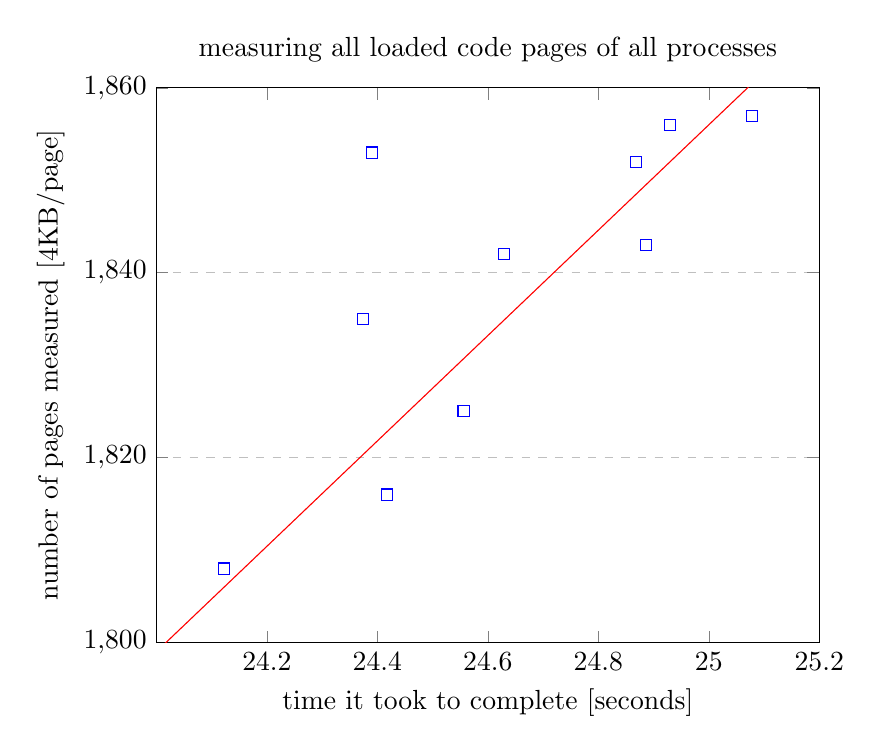
\begin{tikzpicture}
\begin{axis}[
    title={measuring all loaded code pages of all processes},
    xlabel={time it took to complete [seconds]},
    ylabel={number of pages measured [4KB/page]},
    xmin=24, xmax=25.2,
    ymin=1800, ymax=1860,
    xtick={24.2,24.4,24.6,24.8,25,25.2},
    ytick={1800,1820,1840,1860},
    legend pos=north west,
    ymajorgrids=true,
    grid style=dashed,
]

\addplot [
    domain=24:25.2, 
    samples=100, 
    color=red,
]{57*x + 431};

\addplot[
	only marks,
    color=blue,
    mark=square,
    ]
    coordinates {
    (24.868,1852)(24.886,1843)(24.556,1825)(24.930,1856)(24.390,1853)(24.123,1808)(24.417,1816)(24.629,1842)(25.078,1857)(24.374,1835)
    };
    
\end{axis}
\end{tikzpicture}

\paragraph*{}%{One proces}
To provide insight in how long it takes to measure one process (twice) we executed the last experiment on just the \textit{init\_proc} process.

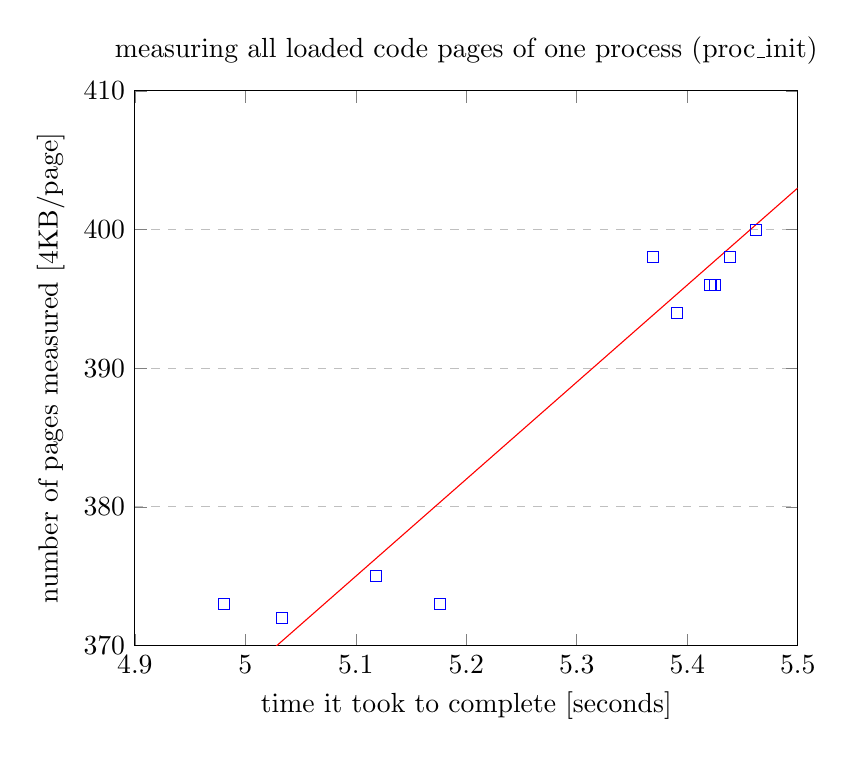
\begin{tikzpicture}
\begin{axis}[
    title={measuring all loaded code pages of one process (proc\_init)},
    xlabel={time it took to complete [seconds]},
    ylabel={number of pages measured [4KB/page]},
    xmin=4.9, xmax=5.5,
    ymin=370, ymax=410,
    xtick={4.9,5,5.1,5.2,5.3,5.4,5.5},
    ytick={370,380,390,400,410},
    legend pos=north west,
    ymajorgrids=true,
    grid style=dashed,
]

\addplot [
    domain=4.9:5.5, 
    samples=100, 
    color=red,
]{70*x + 18};

\addplot[
	only marks,
    color=blue,
    mark=square,
    ]
    coordinates {
    (4.981,373)(5.421,396)(5.369,398)(5.462,400)(5.391,394)(5.033,372)(5.439,398)(5.425,396)(5.118,375)(5.176,373)
    };
    
\end{axis}
\end{tikzpicture}

\paragraph*{}%{One memory region}
In the first two experiments the amount of pages that are loaded into RAM fluctuated a bit, this probably has to do with pages being swapped in and out of memory. In this last experiment only one executable memory region of the \textit{init\_proc} is measured and the amount of pages stays constant for all 10 iterations. The amount of pages measured is 88 and the average execution time is 1.319 seconds, the maximum execution time is 1.353 and the minimum 1.299.

\paragraph*{}
Last but not least the three experiments are plotted in one graph to show how they relate to each other. This plot clearly shows that the amount of time the measurements take is proportional to the amount of pages that are measured. No surprises here because hashing the memory pages is the most compute intensive task of the program but it is good to compare between the different experiments nonetheless. This allows us to compare our achieved performance to that of the paper because we can extrapolate the results to the necessary amount that was measured in the paper.

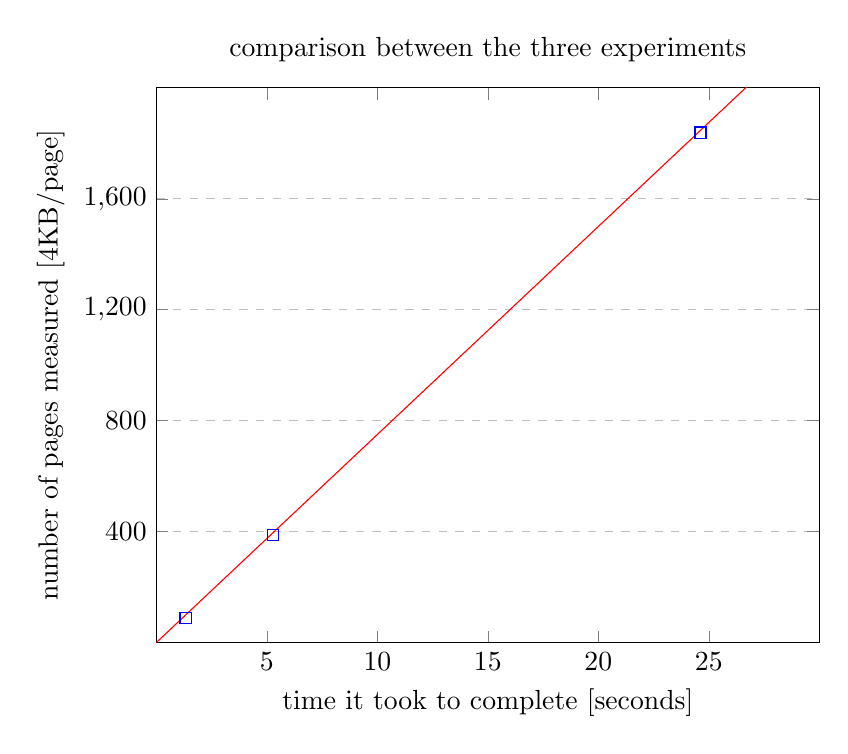
\begin{tikzpicture}
\begin{axis}[
    title={comparison between the three experiments},
    xlabel={time it took to complete [seconds]},
    ylabel={number of pages measured [4KB/page]},
    xmin=0, xmax=30,
    ymin=0, ymax=2000,
    xtick={5,10,15,20,25},
    ytick={400,800,1200,1600},
    legend pos=north west,
    ymajorgrids=true,
    grid style=dashed,
]

\addplot [
    domain=0:30, 
    samples=100, 
    color=red,
]{75*x};

\addplot[
	only marks,
    color=blue,
    mark=square,
    ]
    coordinates {
    (24.625,1839)(5.281,387)(1.319,88)
    };
    
\end{axis}
\end{tikzpicture}

\paragraph*{}%{Comparison}
As can be seen in the three executed experiments, the performance of the implementation of this work is far from that of the paper. Certain aspects are important to highlight which give a partial explanation about the cause of these deviations. First of all the implementation is not written nor fine tuned for performance, it is merely written as a proof of concept. This is due to the restricted amount of time and the lack of experience with making software with high performance. Secondly the memory regions that are attested in this work are only the executable memory pages of a process. These pages need to be identified using multiple files which generally takes more time than in the case that there is one large chunk of memory that is attested. Lastly these experiments are executed on a Qemu emulation of OP-TEE on a general purpose laptop (Lenovo Thinkpad P50) while the experiments in the paper are executed using a hardware prototype. 

\paragraph*{}%{Balance}
While it is hard to make any conclusions based on these pessimistic results, it is useful to elaborate about the balance between performance and added security. A good balance between performance overhead and security assurance depends on the use case. In case of a smart phone we believe even with these results that attesting the executable pages that are loaded in RAM memory every 30 minutes has not too much impact on the user experience. Depending on the amount of newly loaded memory pages when an application is started it could even be considered to attest these pages before starting to execute them. This is a lot more sensitive towards the user experience because this happens while the user is waiting for the application to open, while on the other hand running the attestation in the background on the already loaded pages in RAM should have minimal impact on the user. These considerations do not take into account the energy consumption of running the attestation, because we didn't have the means for these kinds of experiments.

\section{Security Properties}

\paragraph*{}%{}
The attestation method presented in this work focuses on measuring the code pages of processes loaded in RAM. A code page can only gain control or be executed when it is loaded in RAM first. Keeping this prerequisite in mind it should suffice to only attest those pages to ensure no code page that has been tampered with gets to be executed. This last statement of course needs to be loosened a bit because the attestation runs periodically so a code page may have been executed before the changes are noticed by the attestation PTA.

\paragraph*{}%{Integrity of the measurement execution}
Integrity of the measurement execution is of utmost importance when it comes to attestation. In remote attestation the critical code runs on a hardened server which guarantees that it is infeasible to tamper with the execution control flow. In the case of the PinePhone it is not remote attestation we present but user attestation, the critical code which compares the measurements runs in the Secure World. The Trusted Execution Environment provided by ARM TrustZone does guarantee that the Normal World cannot influence the execution of the Secure World in any way as long as the device was started up successfully using secure boot.

\paragraph*{}%{Secure storage of results}
Secure storage of results is very important to have a chance at making remote attestation work. If an adversary were to be able to tamper with these values they could make every attestation attempt fail due to the changed initial value. In case a bad hashing algorithm is chosen and the attacker is able to read the initial hash digest they could also try to forge a collision attack where they tamper with a page in such a way that it's hash digest doesn't change but the code in the page does something the attacker desires. To make sure the reference values are not tampered with they need to be stored in secure memory which should not be accessible from outside the secure world. In the secure world these values should only be written during the initialization phase and afterwards only read. This statement can again be loosened a bit in case there are software updates or additional software to be installed on the device. The initialization phase could be executed again for those code pages and updating or adding the measurement results to the secure storage. 

\section{Security Evaluation}

\paragraph*{}%{Security guarantees}
Security guarantees that can be made are the integrity of the measurement execution control flow and the integrity and confidentiality of the results that are being stored. These are achieved due to secure boot enabling the trusted execution environment of ARM TrustZone. These are key assumptions in the field of remote attestation and thus are also very important in this case of user attestation. Of course when discussing the security guarantees a certain solution offers it is not only about the execution and storage of that application itself but also what additional security guarantees it provides to the system overall. The most important guarantee that an attestation solution tries to provide is being able to detect modifications or unexpected possibly malicious changes to the aspects of the system it attests. In our case the code pages of processes are being attested, we only measure the ones that are present in RAM because only then they are able to do harm to the system. There is still an unsolved problem as also stated in the paper that the rich OS needs to provide the physical addresses of the code pages. This means that malware capable of self hiding or transient root kits are still possible threats that could stay unnoticed to this solution. If an adversary has taken control of the OS there are countless ways in which the attacker could deny the attestation PTA the necessary addresses which at this moment would not result in an attestation alert to the user.

\paragraph*{}%{Shortcomings}
OS/firmware attacks are present in the attacker model of the paper on which this work is based. We believe that with this method the code pages of all processes including those of the rich OS can be attested and this will enable the user to be notified about any tampering with this code base. This does not mean however that tampering with these code pages has become harder and besides tampering with code there are lots of different methods to perform an OS/firmware attack. We believe that this work can be extended upon to thoroughly attest the Normal World (user applications and rich OS) but in it's current state it only allows detection of a small portion of the possible OS/firmware attacks. Even with the problem that the rich OS provides the physical memory addresses solved this incompleteness persists.

\paragraph*{}%{Extensions}
The paper also seems to claim that software attacks are protected against or detectable in the case of attestation. Again in this case we do not think this is a valid statement because the integrity of the code is only a small portion of the attack surface. In this attestation method the data structures are not checked which are the main target for very well known attacks that have been around for decades like buffer overflows and return oriented programming. Extensions to this solution need to be realized to detect software attacks, OS/firmware attacks likewise.
\documentclass{report}

\raggedright

\begin{document}

\chapter{Discussion}

\section{Related work}

\paragraph*{Secure boot, Trusted boot and remote attestation for ARM TrustZone-based IoT Nodes}
is the paper on which the implementation and experiments are based.

\paragraph*{DAA-TZ: An Efficient DAA Scheme for Mobile Devices Using ARM TrustZone}
implements Direct Anonymous Attestation on a mobile ARM TrustZone device.

\paragraph*{SecTEE: A Software-based Approach to Secure Enclave Architecture Using TEE}
implements enclaves on a CPU with ARM TrustZone technology. 

\paragraph*{TZ-MRAS: A Remote Attestation Scheme for the Mobile Terminal Based on ARM TrustZone}
uses ARM TrustZone to protect the attestation service on the mobile device from being tampered with.

\paragraph*{TrustShadow: Secure Execution of Unmodified Applications with ARM TrustZone}
utilizes the functionality of the secure world to shield applications from untrusted OSes.

\section{Comparison of Approaches}

\subsection*{Effectiveness}

\paragraph*{The goal}
of these papers are all a little different but it is important to evaluate which ones actually realized their goal and how this compares to the goal set out by this thesis.

\paragraph*{Most variety of attacks}
that the solution defends against is a clear measure on how effective the solution is in the field.

\paragraph*{The strongest security guarantees}
that were made and achieved also indicate how well the solution works.

\subsection*{Assumptions}

\paragraph*{The least assumptions}
that were made by the authors of the paper the more widely applicable the solution is because there is enormous hetergeneity among devices and assumptions put restrictions on the devices for which the paper is usefull.

\paragraph*{The most realistic assumptions}
are of course also important to look at, if the assumptions are not realistic they are not practical to adhere to and the solution will be worthless if it can't be applied to the real world.

\section{Future Improvements}

\subsection*{Weaknesses}

\paragraph*{Rich OS dependency}
is very undesirable, it is thus important to look at different solutions that achieve similar outcomes to avoid this aspect of the current solution.

\paragraph*{Uncomplete attestation}
introduces a fake sense of security because not all possible attacks are checked, for instance modified data structures that influence the control flow of a program. (inspiration from Lightweight and Flexible Trust Assessment Modules for the Internet of Things)

\subsection*{Additional features}

\paragraph*{•}
Based on the related work papers some additional features could be stated or solutions could be combined to achieve protection against a wider variety of attacks.

\end{document}
\documentclass{report}

\raggedright

\begin{document}

\chapter{Conclusion}

To achieve secure execution on the PinePhone some requirements need to be met. One of these requirements is that a chain of trust is achieved which is done using secure boot in this case.

\section{Contributions}

A detailed process of how to make secure boot happen on a PinePhone using OP-TEE. Besides integrating OP-TEE with the linux operating system of the PinePhone also showing how a secure application can be run from within this setup.
\medskip

An open source implementation of attestation on the PinePhone which allows the Secure World to attest the Normal World and increase the security guarantees thereof.

\section{Future Improvements}

To allow the user to attest their device it is important that Trusted I/O is used to inform the user about the outcome of the attestation process.
\medskip

The attestation application can be seen as one module that can be accompanied with a variety of different modules to increase the amount of checks that can be executed to check more possible attacks/ vulnerabilities.

\end{document}


% If you have appendices:
\appendixpage*          % if wanted
\appendix
%\include{app-A}


\backmatter
% The bibliography comes after the appendices.
% You can replace the standard "abbrv" bibliography style by another one.
\bibliographystyle{ieeetr}
\bibliography{references}

\end{document}

%%% Local Variables: 
%%% mode: latex
%%% TeX-master: t
%%% End: 
